\section{Примеры работы программы}

\subsection{Описание программного решения}

Для решения задачи в среде \textit{MatLab} были написаны функции для каждого требуемого Разделом~1 пункта постановки задачи. Взаимодействие с данными функциями реализуется при помощи интерфейса глобальных переменных, которые принимают условие задачи, а также содержат другие общие для \textit{программного решения} данные. Для удобства использования программного решения реализован графический интерфейс для наиболее часто употребимых функций.

\begin{figure}[h]
\noindent\centering{
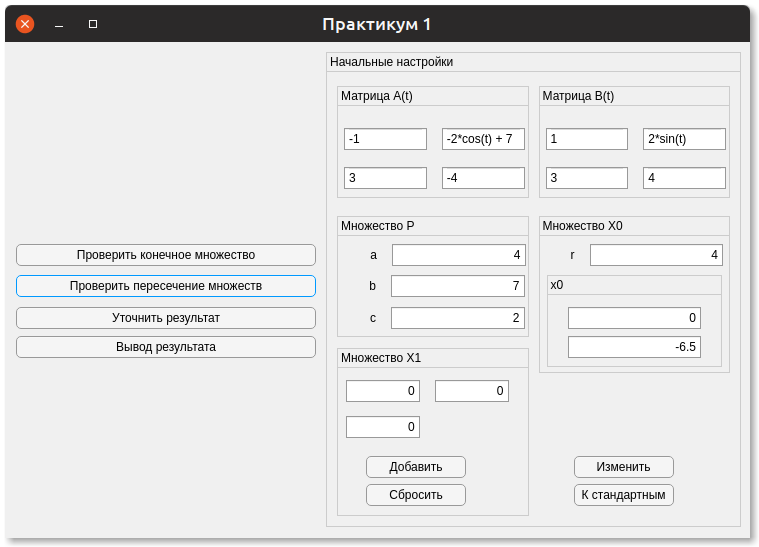
\includegraphics[width=120mm]{program/app.png}
}
\caption{Графический интерфейс программы.}
\label{img:app}
\end{figure}

Далее рассмотрим результаты численного решения задачи для разных начальных данных. Для того, чтобы отличие было более наглядным, зафиксируем начальное, целевое и ограничивающее множества в положении
$$
        B(t) =
        \begin{pmatrix}
                1 & 2\sin t\\
                3 & 4
        \end{pmatrix}, 
$$
$$
        a = 4,\quad b = 7,\quad c = 2,
$$
$$
        x_0 = (-3,\,-7)^\T,\quad r = 4,
$$
$$
        G =
        \begin{pmatrix}
                \;\;\;0{,}3 & \;\;4\\
                -0{,}4 & -2 \\
                \;\;\;0{,}2 & -2
        \end{pmatrix},
        \quad g =
        \begin{pmatrix}
                -10 \\
                \;\;-3 \\
                \;\;-4
        \end{pmatrix}
$$
и обратим внимание на различия численного решения при разных матрицах $A(t)$. Для простоты будем брать константные матрицы $A(t) \equiv A$ с различным типом собственных значений.

\subsection{$A$ с вещественными собственными значениями}